\documentclass[12pt]{article}

\usepackage{graphicx}
\graphicspath{ {Fichier_Image/} }

\title{Batiment optimisé}
\author{Thibault Clodion}

\begin{document}

\maketitle % Permet d'afficher le titre, l'author etc

L'objectif est ici de réaliser un bâtiment dont le temps de sortie est minimale tout en 
respectant le CDC n°1.

\section{Création Générale}

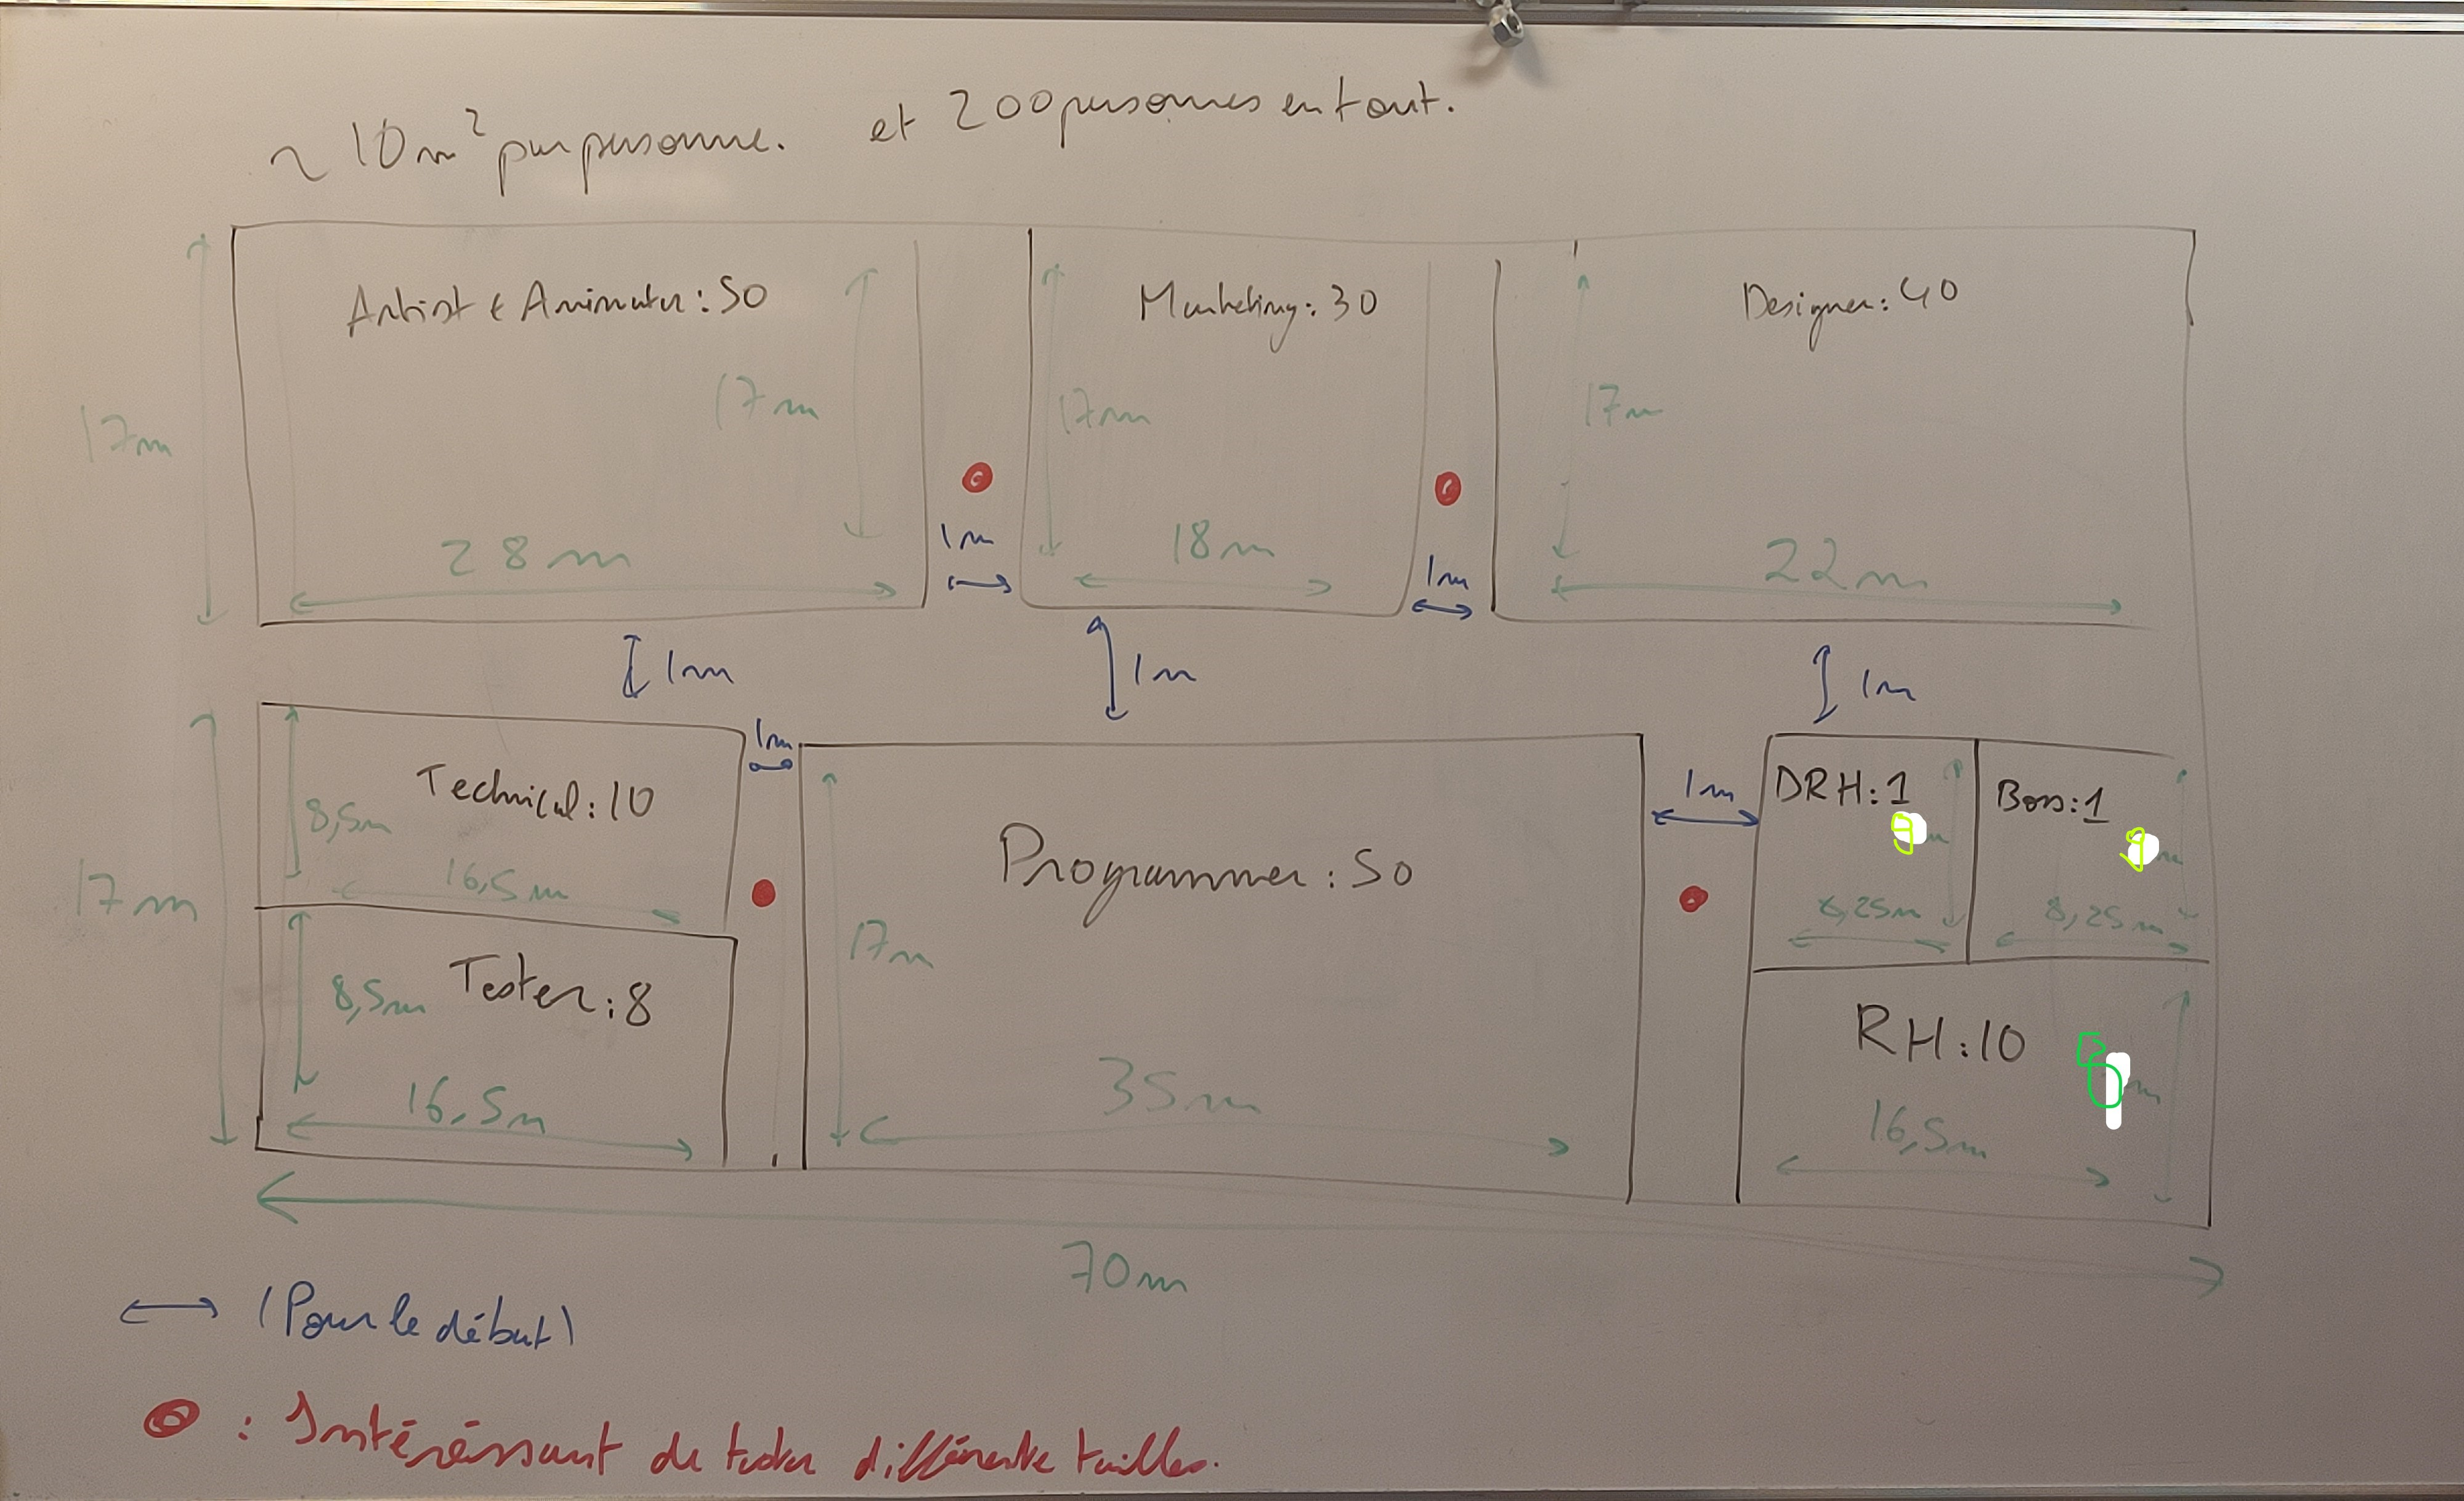
\includegraphics[scale=0.15]{Batiment optimisé croquis.jpg}
\newline\newline
Voici l'allure générale du bâtiment que je vais proposer d'optimiser.
\newline
Au départ il aura rien d'un bâtiment optmisé (couloir 1m, portes mauvais endroits...), mais 
on va montrer que grâce aux hypothèses validés on peut en effet diminuer le temps de sortie moyen.

\section{Premier Batiment}
On va reproduire le bâtiment sous sa forme non optimisé pour faire nos premières observations sur ce dernier.
\newline\newline
La photo ci-dessous montre le bâtiment dans sa phase originale (sans aucune optimisation et classique)
\newline
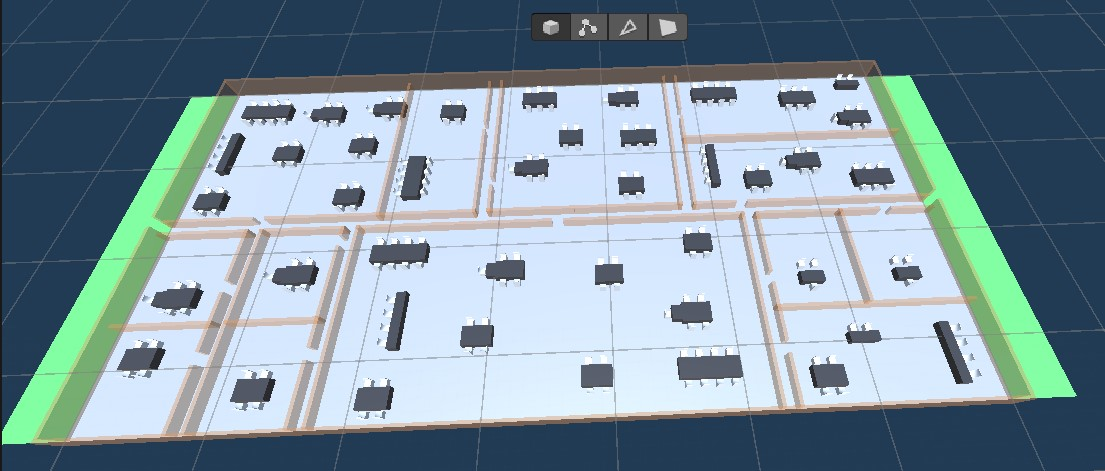
\includegraphics[scale=0.5]{Batiment initial.jpg}
\newline\newline
Temps moyen de dernière sortie : 29.46

\section{Application des hypothèses}
\subsection{Hypothèse 3. : nombre de portes}
On peut remarquer que l'Hypothèse 3. n'est pas respecté à plusieurs endroits dans le bâtiment
\newline
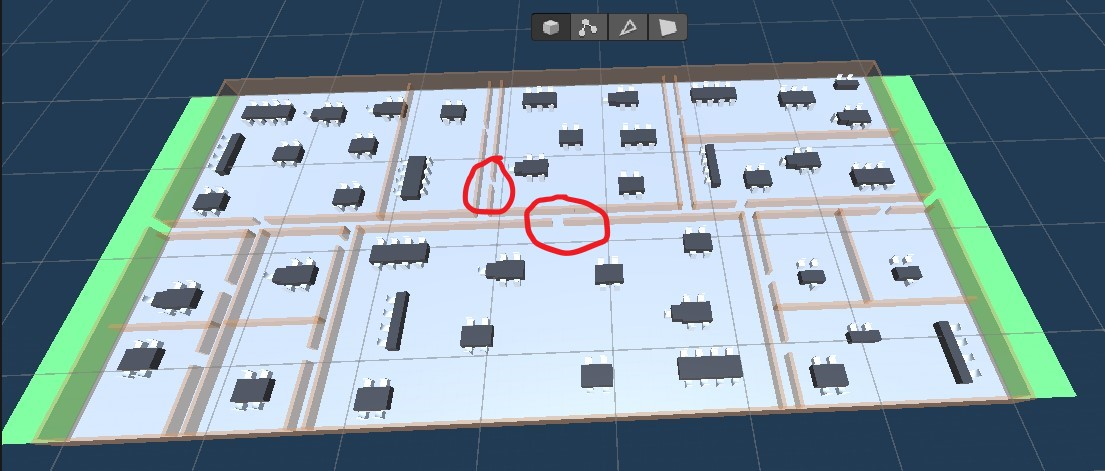
\includegraphics[scale=0.5]{Batiment problème 3..jpg}
\newline
Il faut en effet que les bureaux situés au milieux ait plusieurs portes.
\newline\newline
Après application de l'hypothèse on obtient le bâtiment suivant :
\newline
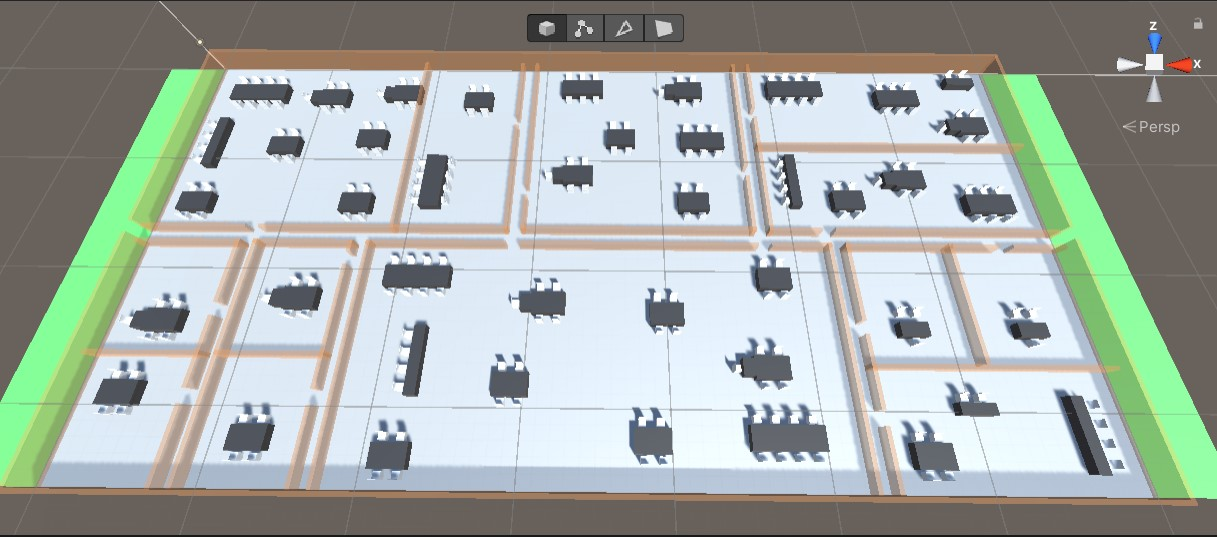
\includegraphics[scale=0.5]{Batiment Hypothèse 3..jpg}
\newline\newline
Remarque
\begin{itemize}
    \item On n'observe plus aucun flux croisé au milieu du bâtiment
    \item La densité du flux dans les zones en rouge est divisé par deux (grâce aux 2 portes rajoutés)
    \item La fluidité de la sortie est nettement amélioré
    \item Il est clair que le nombre de portes joue un rôle crucial ! 
\end{itemize}
Temps moyen de dernière sortie : 25.43
\subsection{Hypothèse 5. : taille des bureaux}
On peut remarquer qu'à un endroit, l'hypothèse 5 n'est pas vérifié
\newline
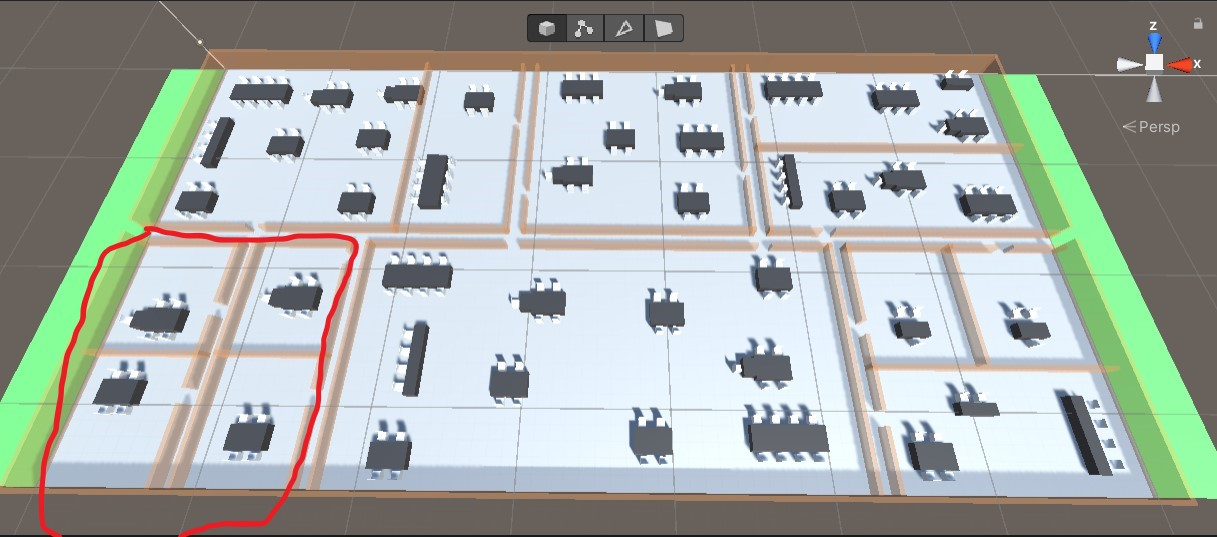
\includegraphics[scale=0.5]{Batiment problème 5..jpg}
\newline
\begin{itemize}
    \item Le changement est assez minime 
    \item Cependant on peut remarquer que c'est plutôt fluide dans la zone identifié
    \item Cela ne peut de toute manière pas être négatif
\end{itemize}
Temps moyen de dernière sortie : 25.36
\subsection{Hypothèse 6. : Croisements}

L'hypothèse 6 n'est pas vérifié à pleins d'endroits différents !
\newline
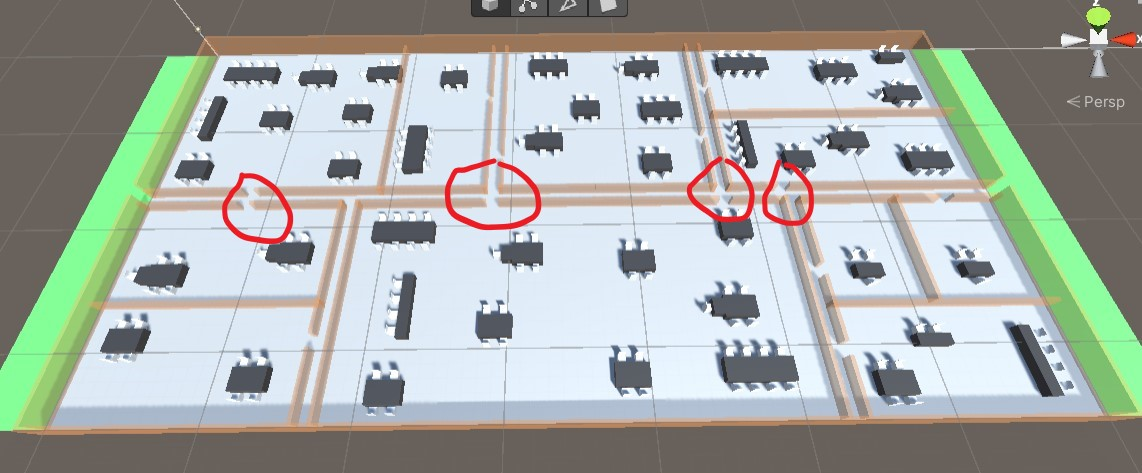
\includegraphics[scale=0.5]{Batiment problème 6..jpg}
\newline
\begin{itemize}
    \item Il est plus simple de modifier l'emplacement des portes que des couloirs, d'où les modifications faites.
    \item On peut également rapprocher quelques portes de la sortie pour ne pas que les personnes aient à faire des détours.
\end{itemize}
On obtient alors le bâtiment suivant.
\newline
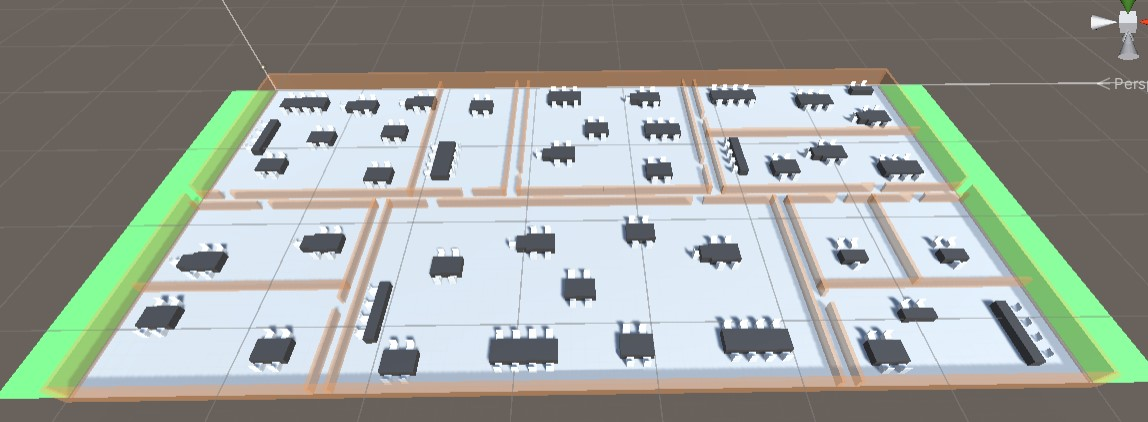
\includegraphics[scale=0.5]{Batiment Hypothèse 6..jpg}
\newline
\begin{itemize}
    \item On a beaucoup moins de collisions, et une division du flux.
    \item Cependant on peu constater que à chaque simulation ce sont les personnes dans le bureaux du milieu bas qui sortent en dernier c'est donc améliorable.
\end{itemize}
Temps moyen de dernière sortie : 22.83s
\subsection{Hypothèse 1. : Taille des couloirs}
Cette hypothèse nous donne le fait qu'il faut que tous les couloirs soit un peu plus grand que les portes de sorties
(le meilleur trouvé etant tous les couloirs à 1m25)
\newline\newline
On modifie alors tous les couloirs de sortent à ce qu'ils fassent 1m25 de large.
\newline\newline
On obtient le bâtiment suivant :
\newline
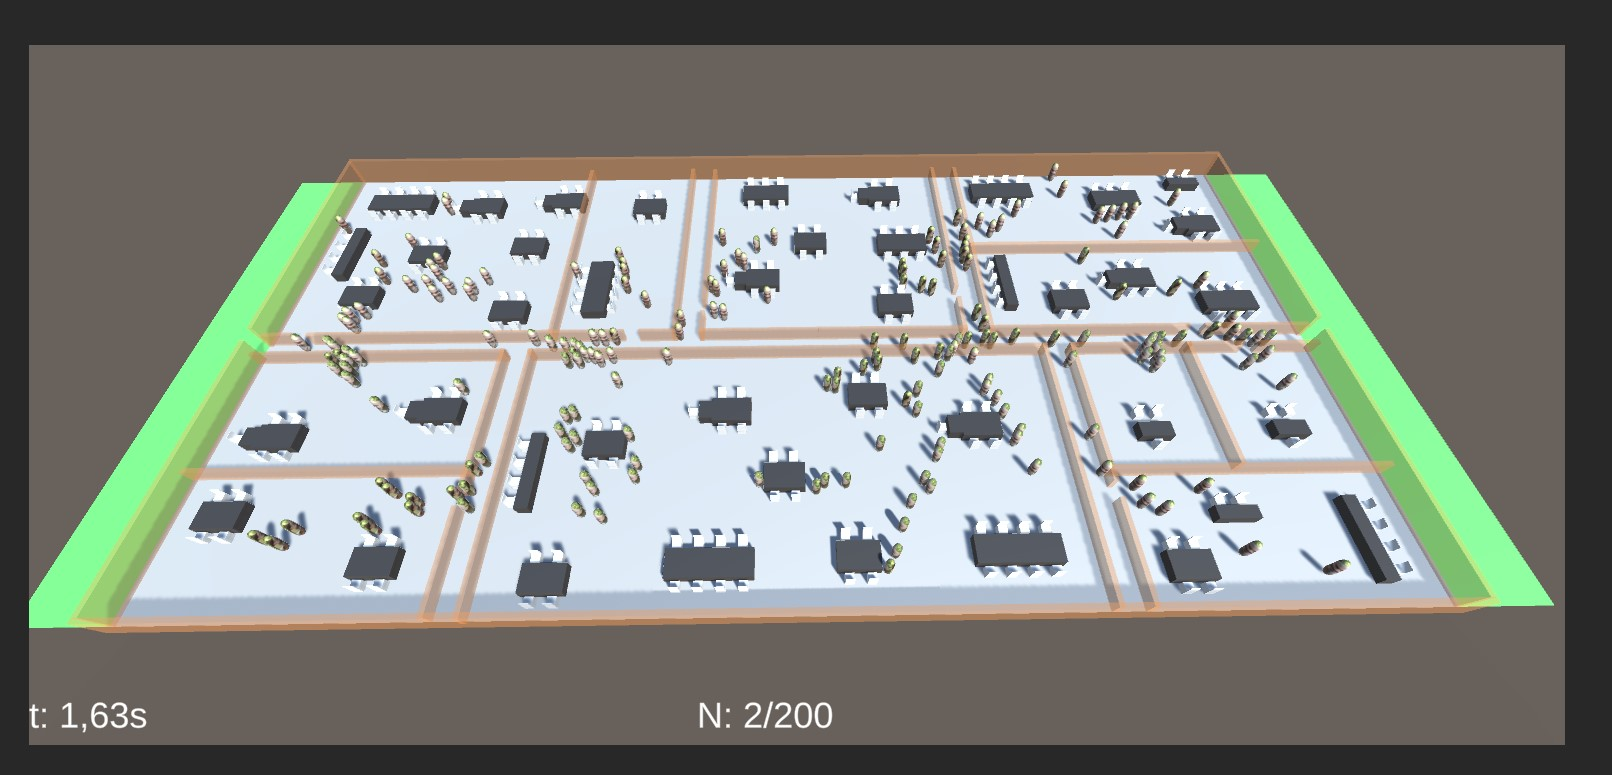
\includegraphics[scale=0.5]{Batiment Hypothèse 1..jpg}
\newline
\begin{itemize}
    \item
\end{itemize}
Temps moyen de dernière sortie : 22.22s
\subsection{Resultats}
Les hypothèses sont en effet cohérentes.
\newline
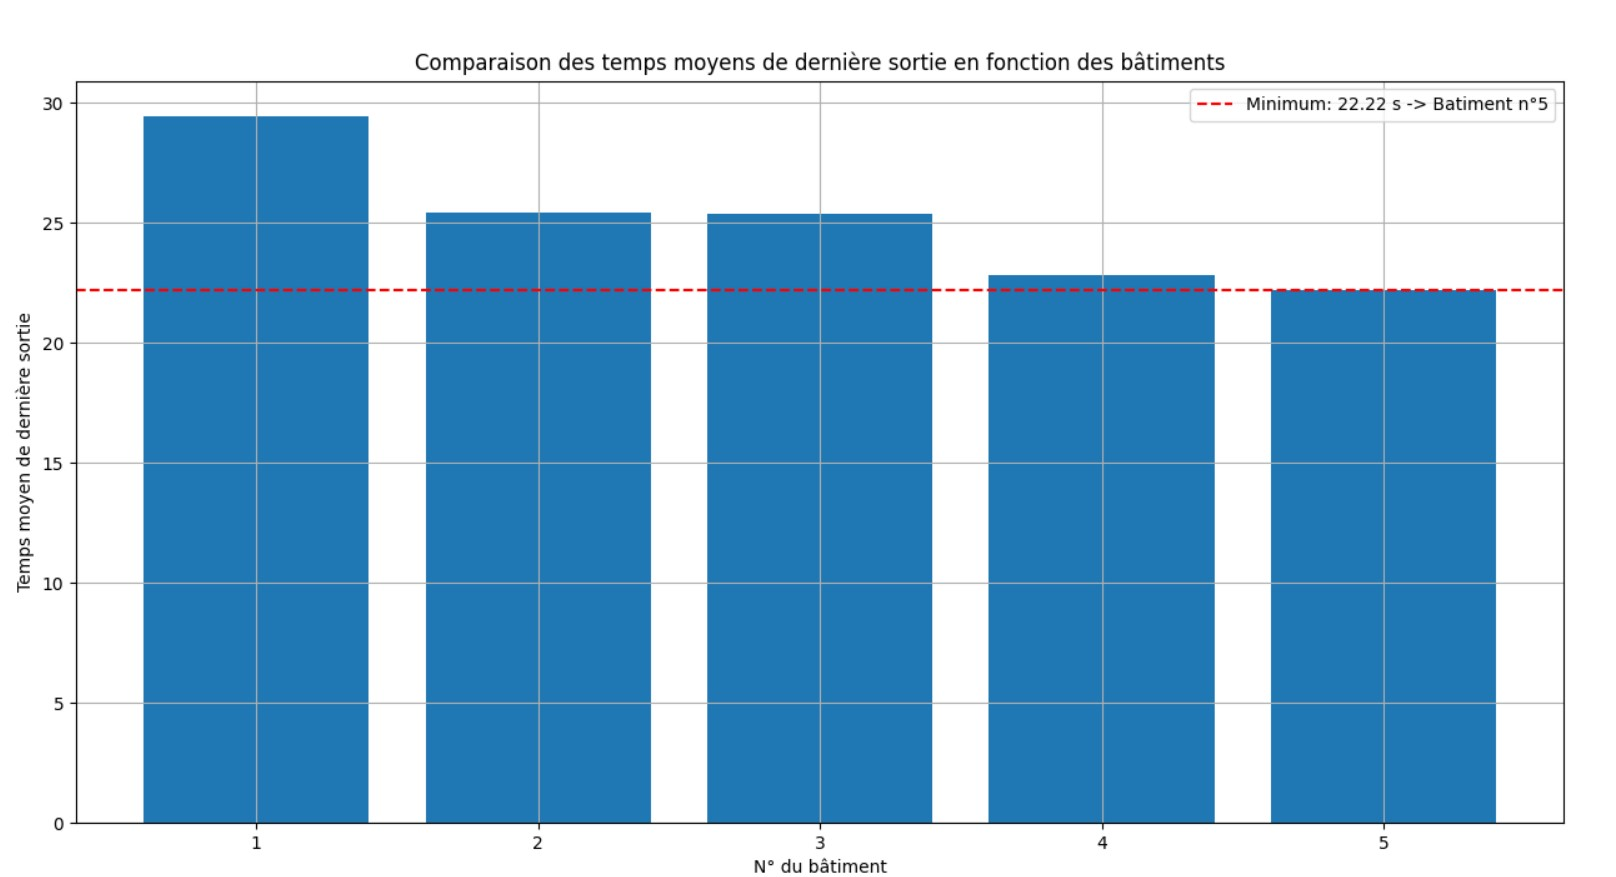
\includegraphics[scale=0.4]{Resultat - Hypothese.jpg}
\newline

\section{Micro-optimisation spécifiques au bâtiment}

On peut remarquer que les hypothèses ont permis de réduire le temps de sortie mais il est sûrement possible d'améliorer encore quelques petits trucs.

\subsection{}
On va tenter de résoudre le problème suivant : Les derniers à sortir sont toujours ceux aux bureaux du mileu bas car il est trop grand et
donc le flux à ces portes est trop important.
\newline
Le nouveau bâtiment est le suivant :
\newline
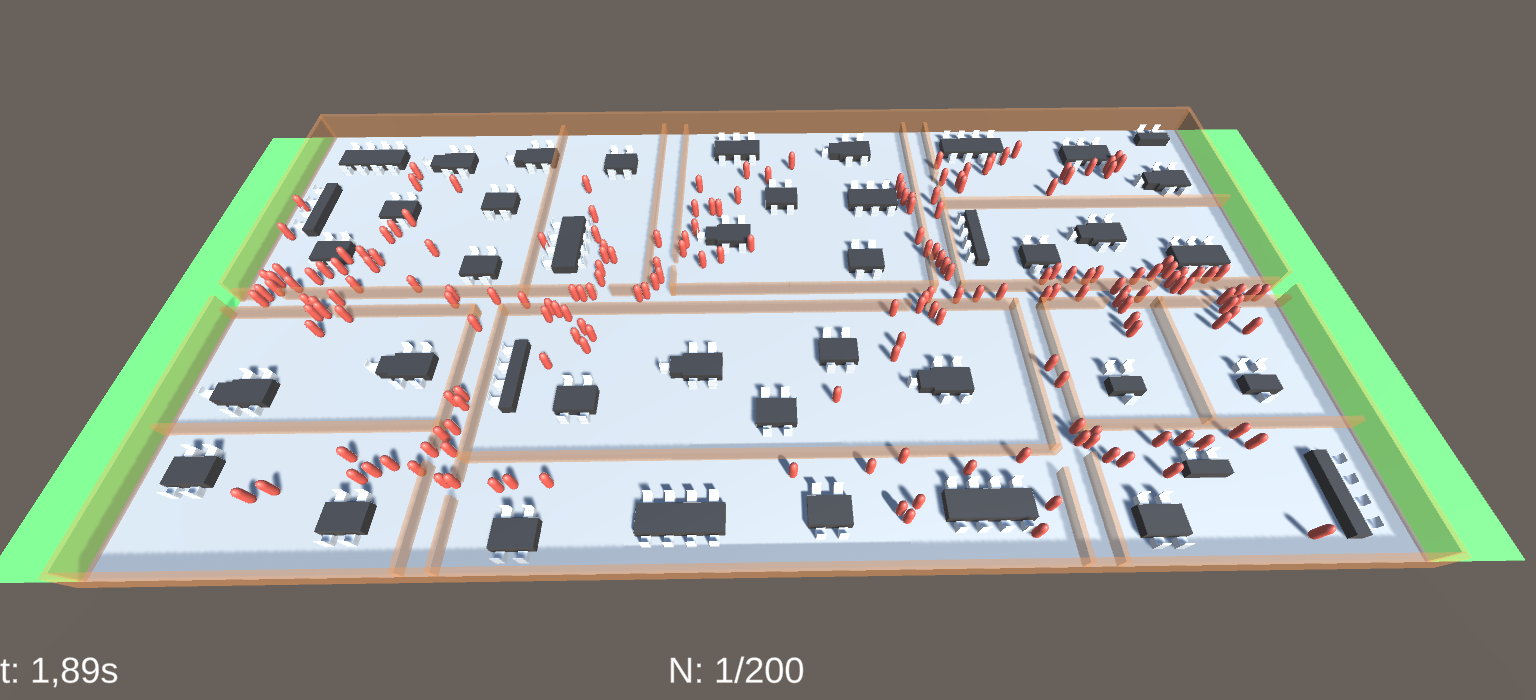
\includegraphics[scale=0.3]{Batiment 4.1 - Visuel.png}
\newline
Le fait d'avoir diviser le bureau en deux fait qu'on a moins de flux au niveau des portes de sorties du bureau
\newline\newline
Temps moyen de sortie obtenu : 21.67s (donc bien mieux)

\subsection{}
On observe que souvent les personnes qui suivent le chemin en bleu sortent en dernier car ils doivent faire un grand detour.
\newline
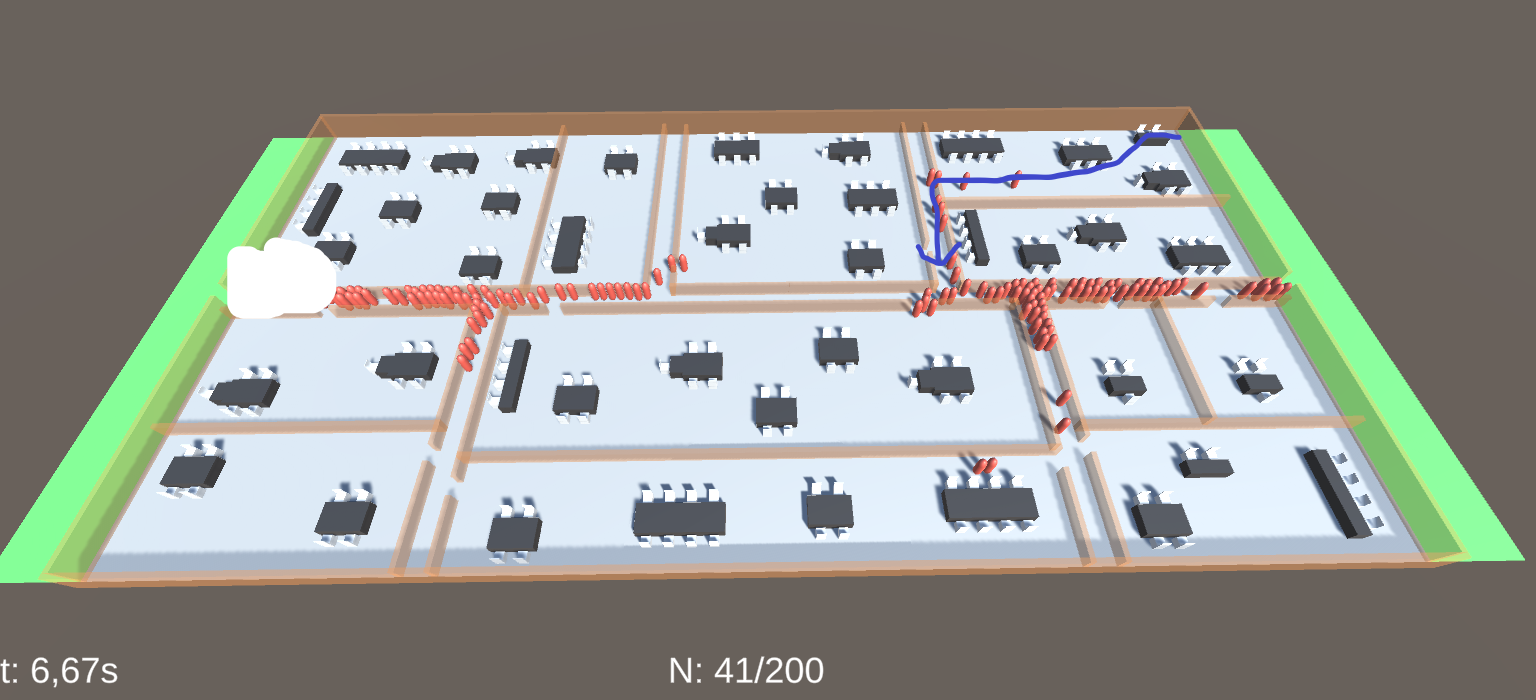
\includegraphics[scale=0.3]{Batiment 4.1 - Problème.png}
\newline
On règle ce problème de la manière suivante : 
\newline
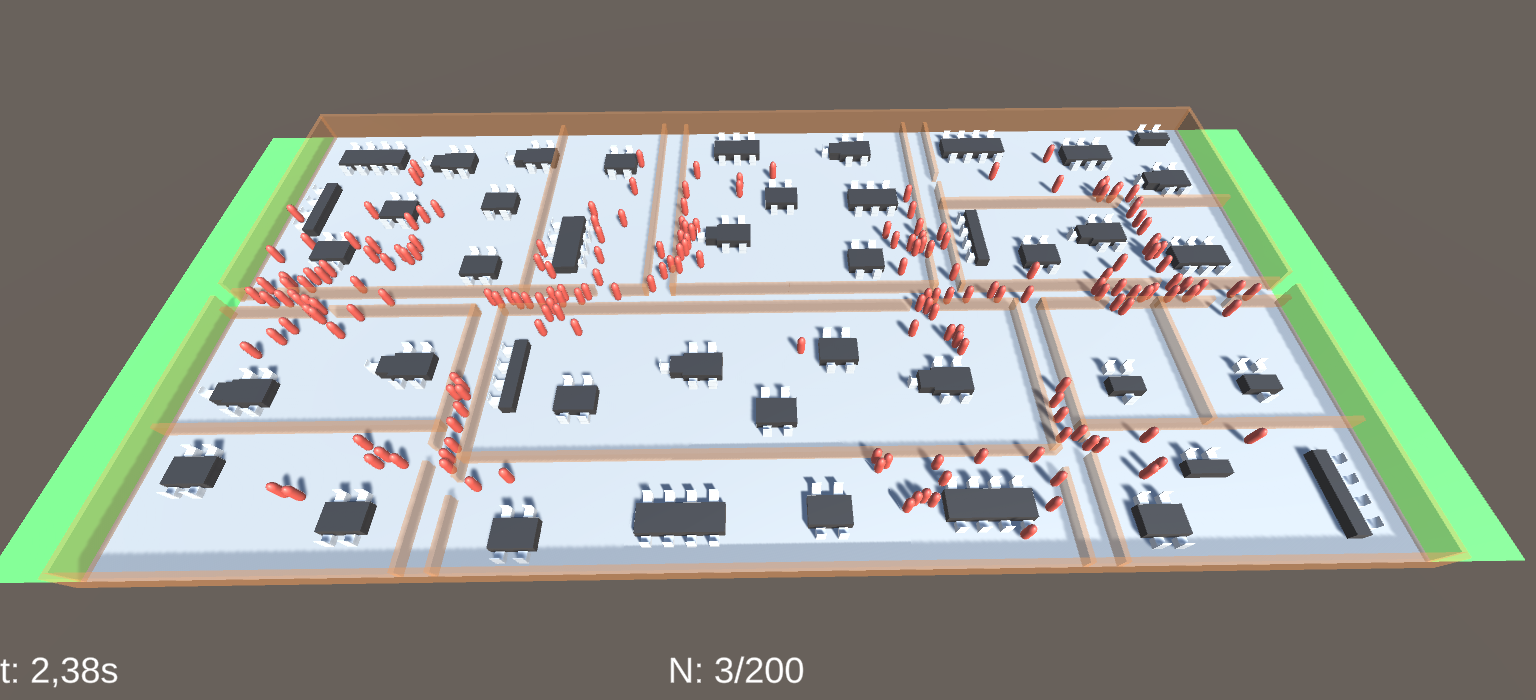
\includegraphics[scale=0.3]{Batiment 4.2 - Visuel.png}
\newline
On obtient le temps moyen suivant : 20.59s (c'est encore mieux)

\section{Conclusion efficacité de l'optimisation}
Cette section a pour but de comprendre ce que l'optimisation a apporter en réalité.
\newline\newline
\subsection{Temps}
Avec seulement l'application des hypothèses :
\begin{itemize}
    \item Temps moyen de sortie : de 29.46 à 22.22s
    \item Temps minimale obtenue : de 22.82 à 18.53s
    \item Temps Maximale obtenue : de 34.70s à 27.88s
\end{itemize}

\subsection{En Terme de Vie}
Cette section a pour but de representer ce que la différence de temps représente en terme de vie sauvé.
\newline\newline
En applicant les hypothèses on a gagné 7.24s sur le temps de sortie moyen
\newline\newline
Cela représente :
\begin{itemize}
    \item Nombre de personnes non sauvés en moyenne : 18.17
    \item Nombre de personnes non sauvés en pourcentage : 9\% (ce qui est proche de ce que j'ai trouvé lors de la MCOT, et de la Bibliographie commenté)
\end{itemize}
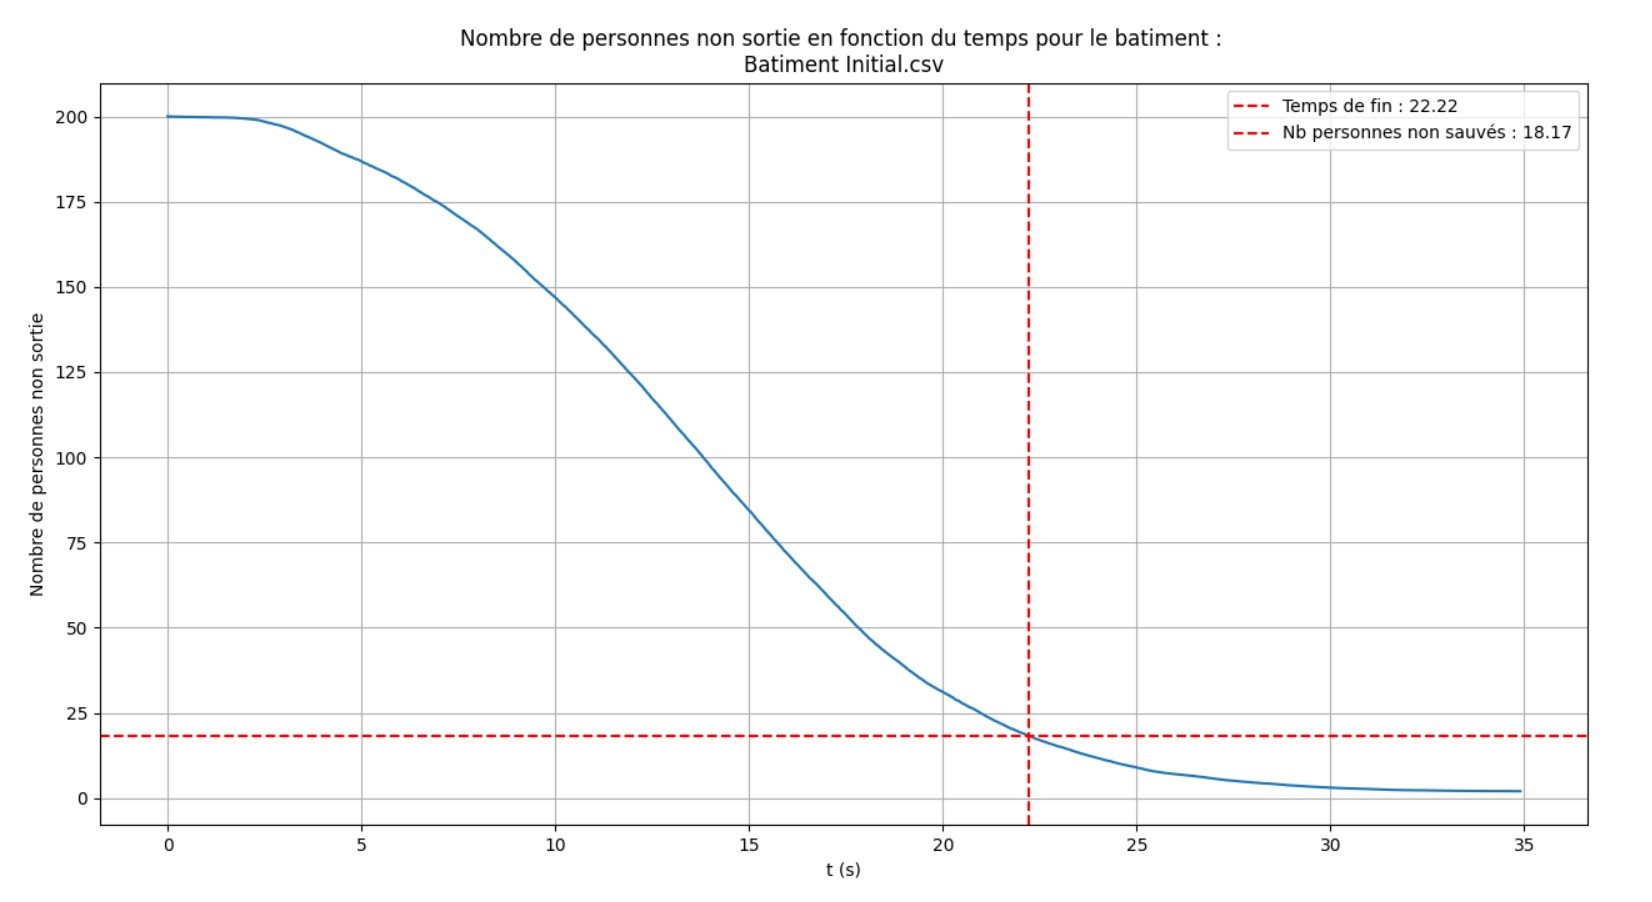
\includegraphics[scale=0.5]{Nombre_personnes_non_sauve.jpg}
\newline
\subsection{}
Les hypothèses ont donc l'air concluante, chacune ont permis de baisser le temps moyen de sortie. Et on se 
retrouve au final à avoir gagné 7.24 secondes sur le temps de sortie moyen ce qui représente dans le batiment inital 18.17 
personnes qui ne seraient pas sorties.


\end{document}